\section{The slave instance}

\begin{wrapfigure}{r}{0.4\textwidth}
  \vspace{-20pt}
  \begin{center}
    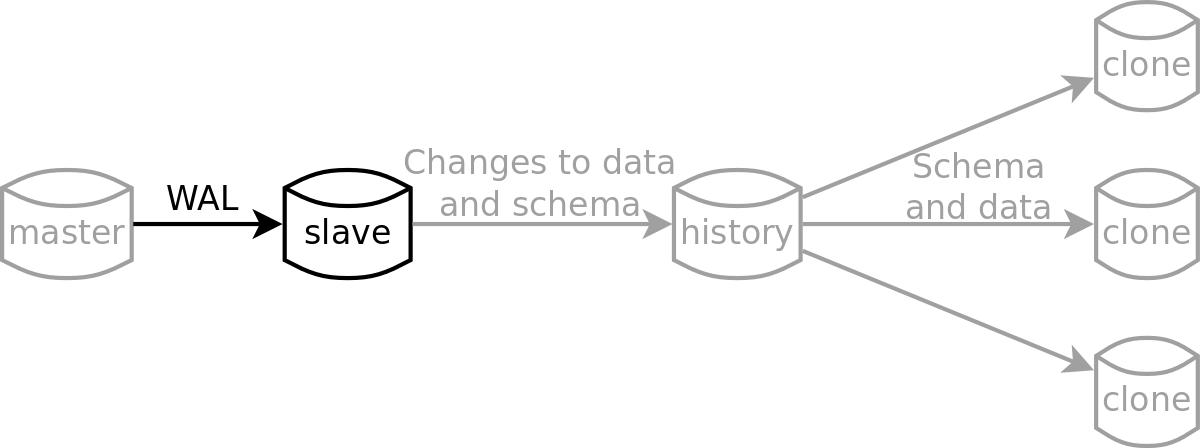
\includegraphics[width=0.38\textwidth]{img/architecture-slave}
  \end{center}
  \vspace{-20pt}
  \caption{The slave part of the architecture}
  \vspace{-10pt}
\end{wrapfigure}

Marty uses the slave instance to initialize the history database and to inspect the contents of the write-ahead log from the master.
The slave is configured to act as a \textit{hot standby} for the master; it starts with a copy of the master database and updates it with the WAL.
When the slave database is first started Marty copies its schema and data to the history database.
It then inspects the changes from the WAL as they are applied and updates the history database accordingly.

Before the slave instance is started a database administrator must configure the master.
This includes configuring a few parameters in the \textit{postgres.conf} file, see table \ref{tbl:master-config}.
Next the administrator must create a \textit{base backup} of the master database.
A base backup is a copy of the cluster files that store all the data in the database.
It can be created with the program \textit{pg\_basebackup} and might require changes to the \textit{pg\_hba.conf} file, see the Postgres documentation for further reference. % TODO add referernce?

\begin{table}[h]
  \centering
  \texttt{
    \begin{tabular}{| l | l |}
      \hline
      \textbf{Parameter} & \textbf{Value} \\ \hline
      wal\_level & hot\_standby \\ \hline
      archive\_mode & on \\ \hline
      archive\_command & 'cp \%p /path/to/archive/\%f' \\ \hline
      max\_wal\_senders & 1 \\ \hline
    \end{tabular}
  }
  \caption{Configuration parameters in postgres.conf for the master database}
  \medskip
  \small
  The archive command is an example, when the master is configured it must use an archive command that copies the WAL files to a storage where they are accessible by the slave.
  Also note that \texttt{max\_wal\_senders} must at least be 1, but can be higher.
  \label{tbl:master-config}
\end{table}

As previously noted the slave runs on a patched version of Postgres that must be compiled with a special flag that enables Postgres to log the WAL replay actions.
When the patch has been applied to the Postgres source code it must be compiled with the \texttt{WAL\_DEBUG} CPP flag.

Instead of creating a new database cluster for the slave with the \texttt{initdb} command the administrator uses the base backup from the master.
When it has been copied to the correct place the \textit{postgres.conf} file must be updated, see table \ref{tbl:slave-config}.
It is then necessary to add a \textit{recovery.conf} file with a command to fetch the WAL files from the master database, see the Postgres documentation for further reference. % TODO reference?

\begin{table}[h]
  \centering
  \texttt{
    \begin{tabular}{| l | l |}
      \hline
      \textbf{Parameter} & \textbf{Value} \\ \hline
      hot\_standby & on \\ \hline
      wal\_debug & on \\ \hline
    \end{tabular}
  }
  \caption{Configuration parameters in postgres.conf for the slave database}
  \label{tbl:slave-config}
\end{table}

\subsection{Reading the WAL}
The write-ahead log contains all the changes that are applied to the master database.
They are stored in binary records that can be applied directly to the files in the slave database cluster to repeat the changes on the slave.
There are a few different kinds of WAL records that store information about different operations on the master.
The ones that Marty looks for are \textit{heap} records and \textit{commit} records.

Heap records contain changes to the tables in the database; inserts, updates and deletes.
The commit records signal the slave to commit and close the current transaction that is being replayed from the WAL.
Other kinds of WAL records include B-tree records for B-tree indexes and XLOG records that contain information about transaction logs.

Marty can read information about the heap records in the WAL replay log.
The log contains information such as the type of the heap record; insert, update or delete, and identifiers of the database and table that the record alters.
The log also contains references to the row which was inserted, updated or deleted.

\begin{lstlisting}[caption={WAL replay log example},label={lst:wal-replay-log},numbers=left,xleftmargin=2em]
LOG:  REDO @ 0/800F1A0; LSN 0/800F248: prev 0/800F160; xid 741; len 139: Heap - insert: rel 1663/16384/11829; tid 39/63
LOG:  REDO @ 0/900390C; LSN 0/9003944: prev 0/9002158; xid 742; len 26: Heap - delete: rel 1663/16384/11829; tid 39/38 KEYS_UPDATED
LOG:  REDO @ 0/8011D80; LSN 0/8011F0C: prev 0/8011D54; xid 741; len 368: Transaction - commit: 2014-03-06 23:36:33.937958+00; inval msgs: catcache 59 catcache 58 catcache 59 catcache 58 catcache 45 catcache 44 catcache 7 catcache 6 catcache 7 catcache 6 catcache 7 catcache 6 catcache 7 catcache 6 catcache 7 catcache 6 catcache 7 catcache 6 catcache 7 catcache 6 relcache 16394
\end{lstlisting}

Listing \ref{lst:wal-replay-log} has an example of the WAL replay log.
The insert and delete heap records in lines 1 and 2 in this example alter the same table.
This table can be looked up with the \textit{rel} values in the log; 1663 is the database ID, 16384 is the namespace ID and 11829 is the table ID.
Marty uses the database and table IDs to look up the table in the slave database and queries it with the \textit{tid} values, which in this case are 39/63 and 39/38.
The tid values reference the row which was inserted to or deleted from the table.
The last line of the example, line 3, logs a commit record.
It closes the transaction and applies the changes from lines 1 and 2 to the slave database.

The next section describes the schema of the history database and how Marty queries the slave database for data to insert into the history.